
	\begin{enumerate}
		\item Дата собрания: 24.10.14
		\item Цель:
		\begin{itemize}
			\item Установить одно опорное колесо вместо двух
			\item Попробовать мебельные стяжки в качестве креплений балочных элементов подъемника
			\item Проверить подвижность робота
		\end{itemize}			
		\item Результаты:
		\begin{itemize}
			\item Приводные колеса робота были отодвинуты назад примерно на 5см, так как робот очень часто вставал на задние колеса и переворачивался
			\item Стяжки хорошо проявили себя в качестве креплений: они не создают почти никакого трения, при этом сохраняя стабильность конструкции
			\item Робот оказался довольно подвижным, забирается на пандус, разворачивается на нем и спускается без проблем
			\item Программа была написана для максимально легкого управления
		\end{itemize}
		\item Идеи и планы:
		\begin{itemize}
			\item Оставить колесную базу в покое и начать строить только подъемник
		\end{itemize}
		\begin{figure} [h]
			\centering
			\begin{minipage}{0.3\linewidth}
				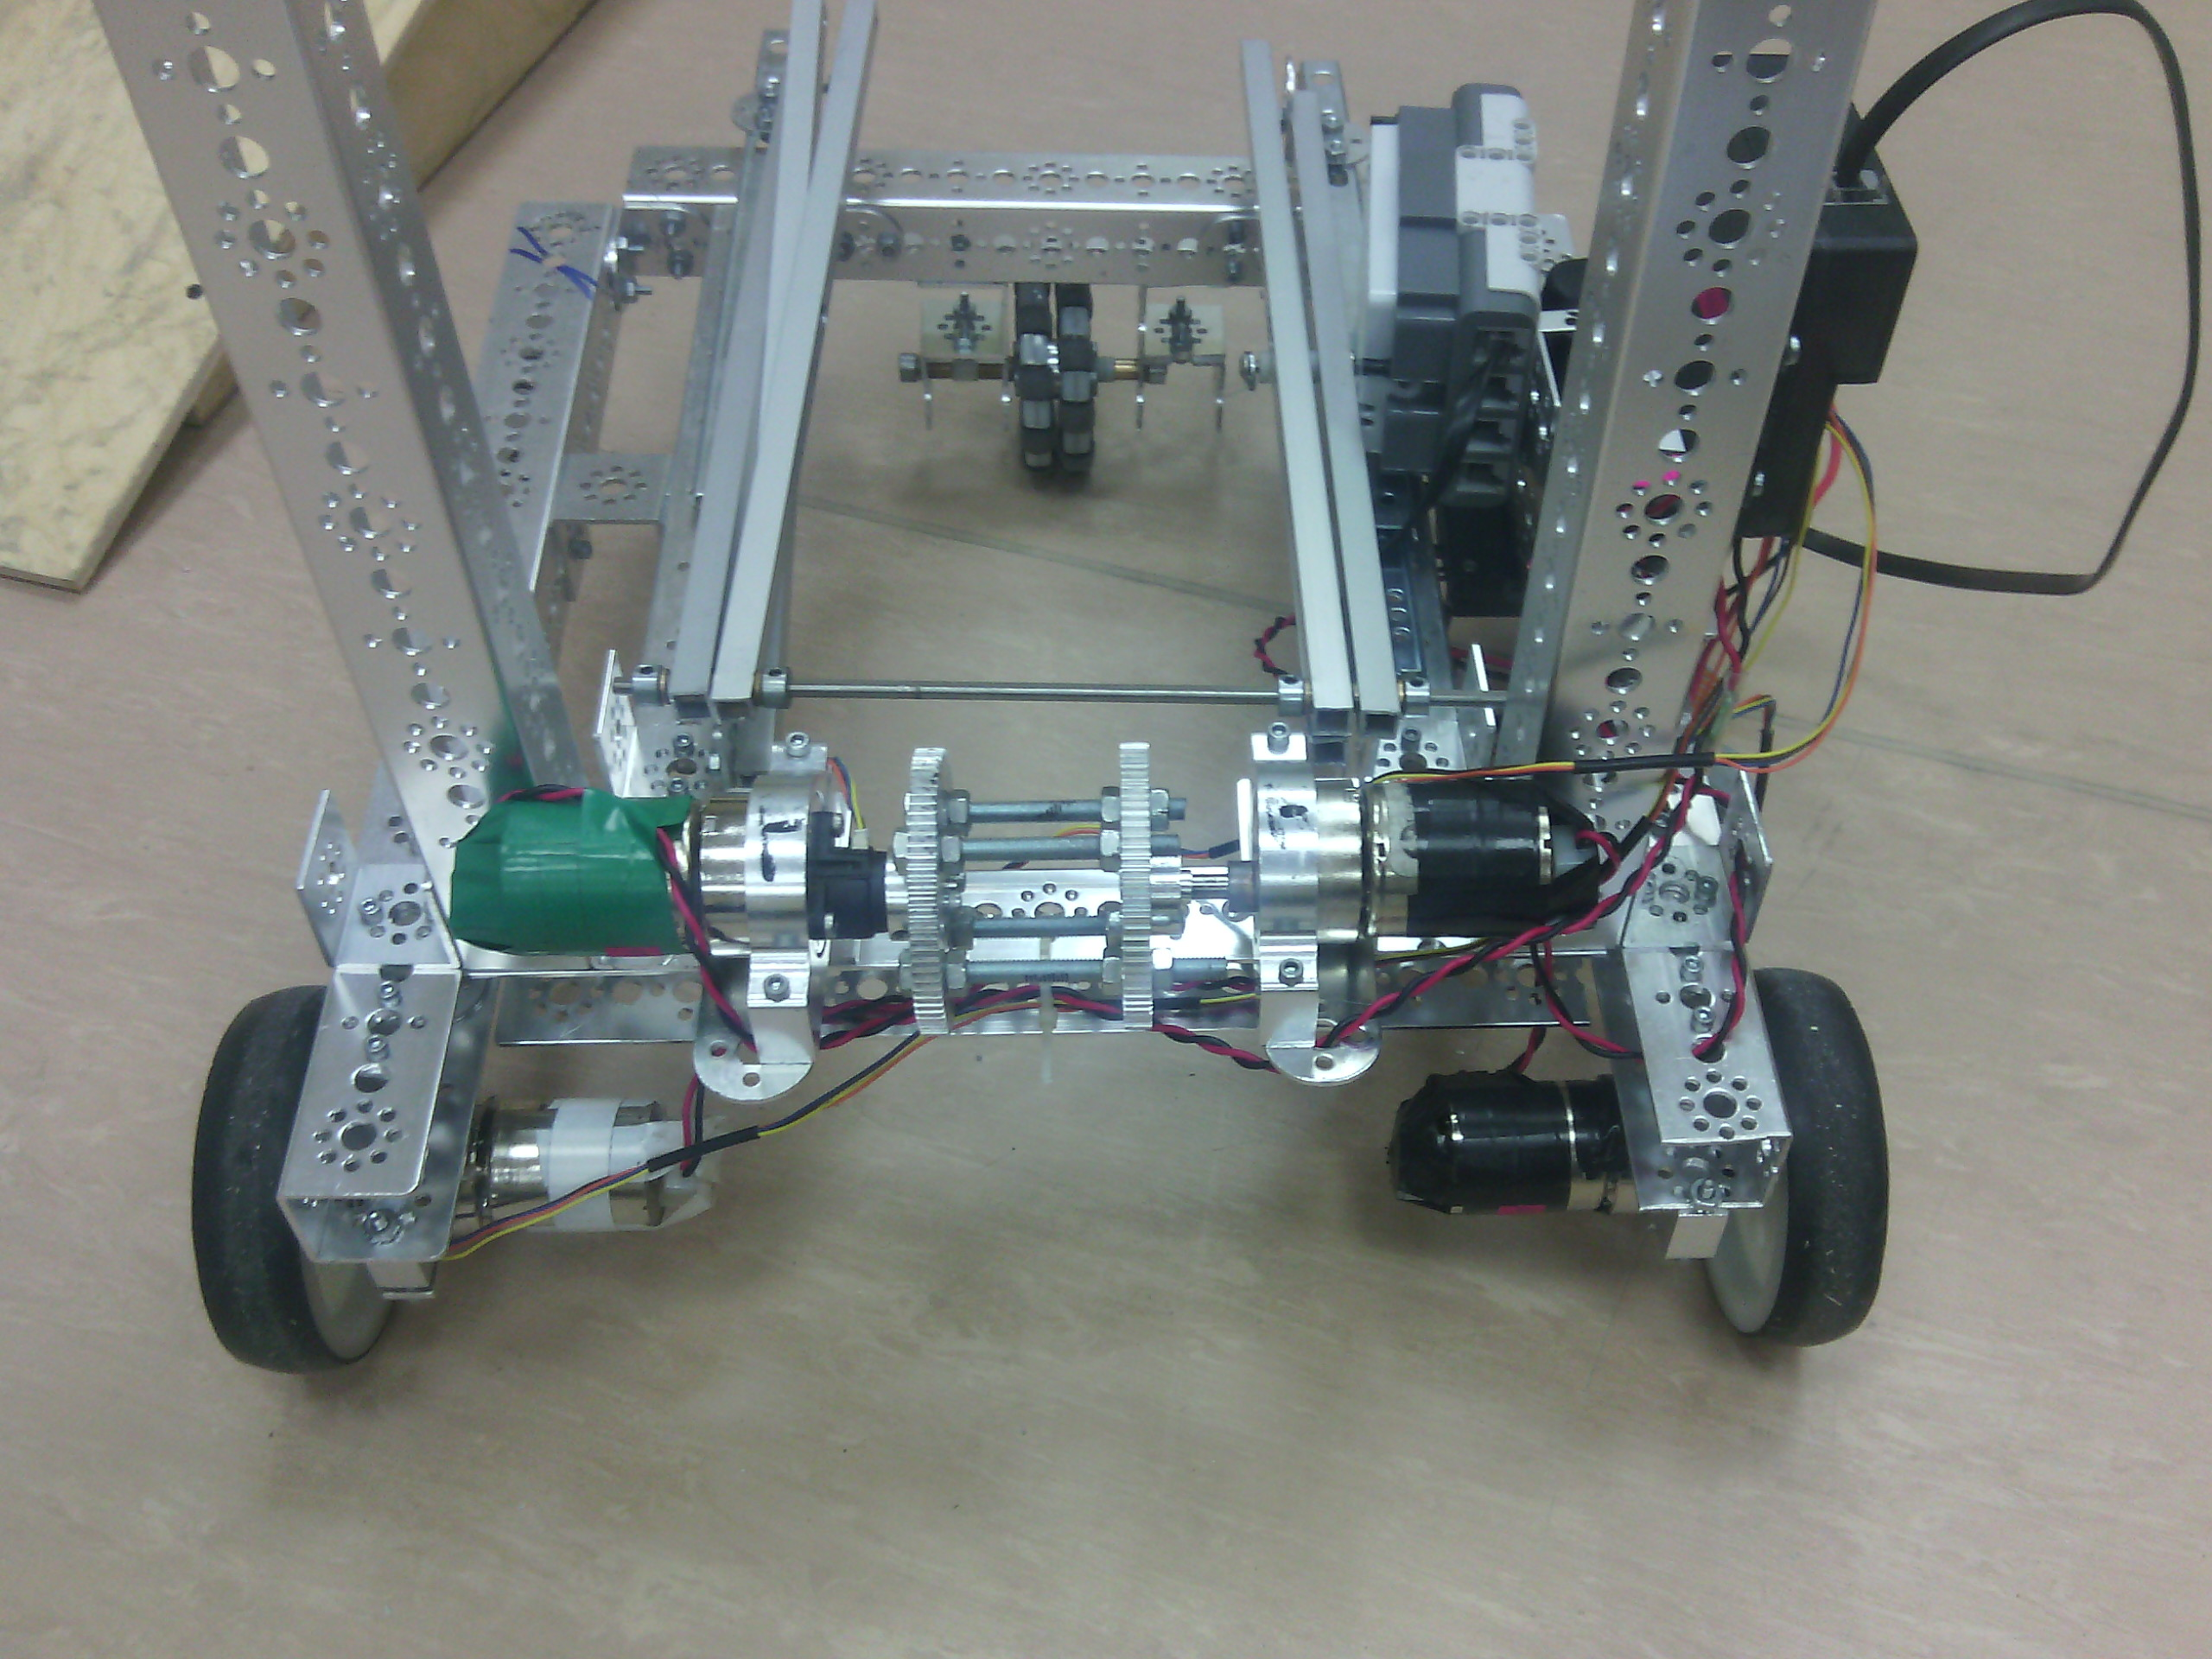
\includegraphics[width=35mm,height=35mm]{/!my_data/projects/pml30-psi_team/Days/24.10.14/9_1_robot}\\ Рисунок 11
			\end{minipage}
			\begin{minipage}{0.3\linewidth}
				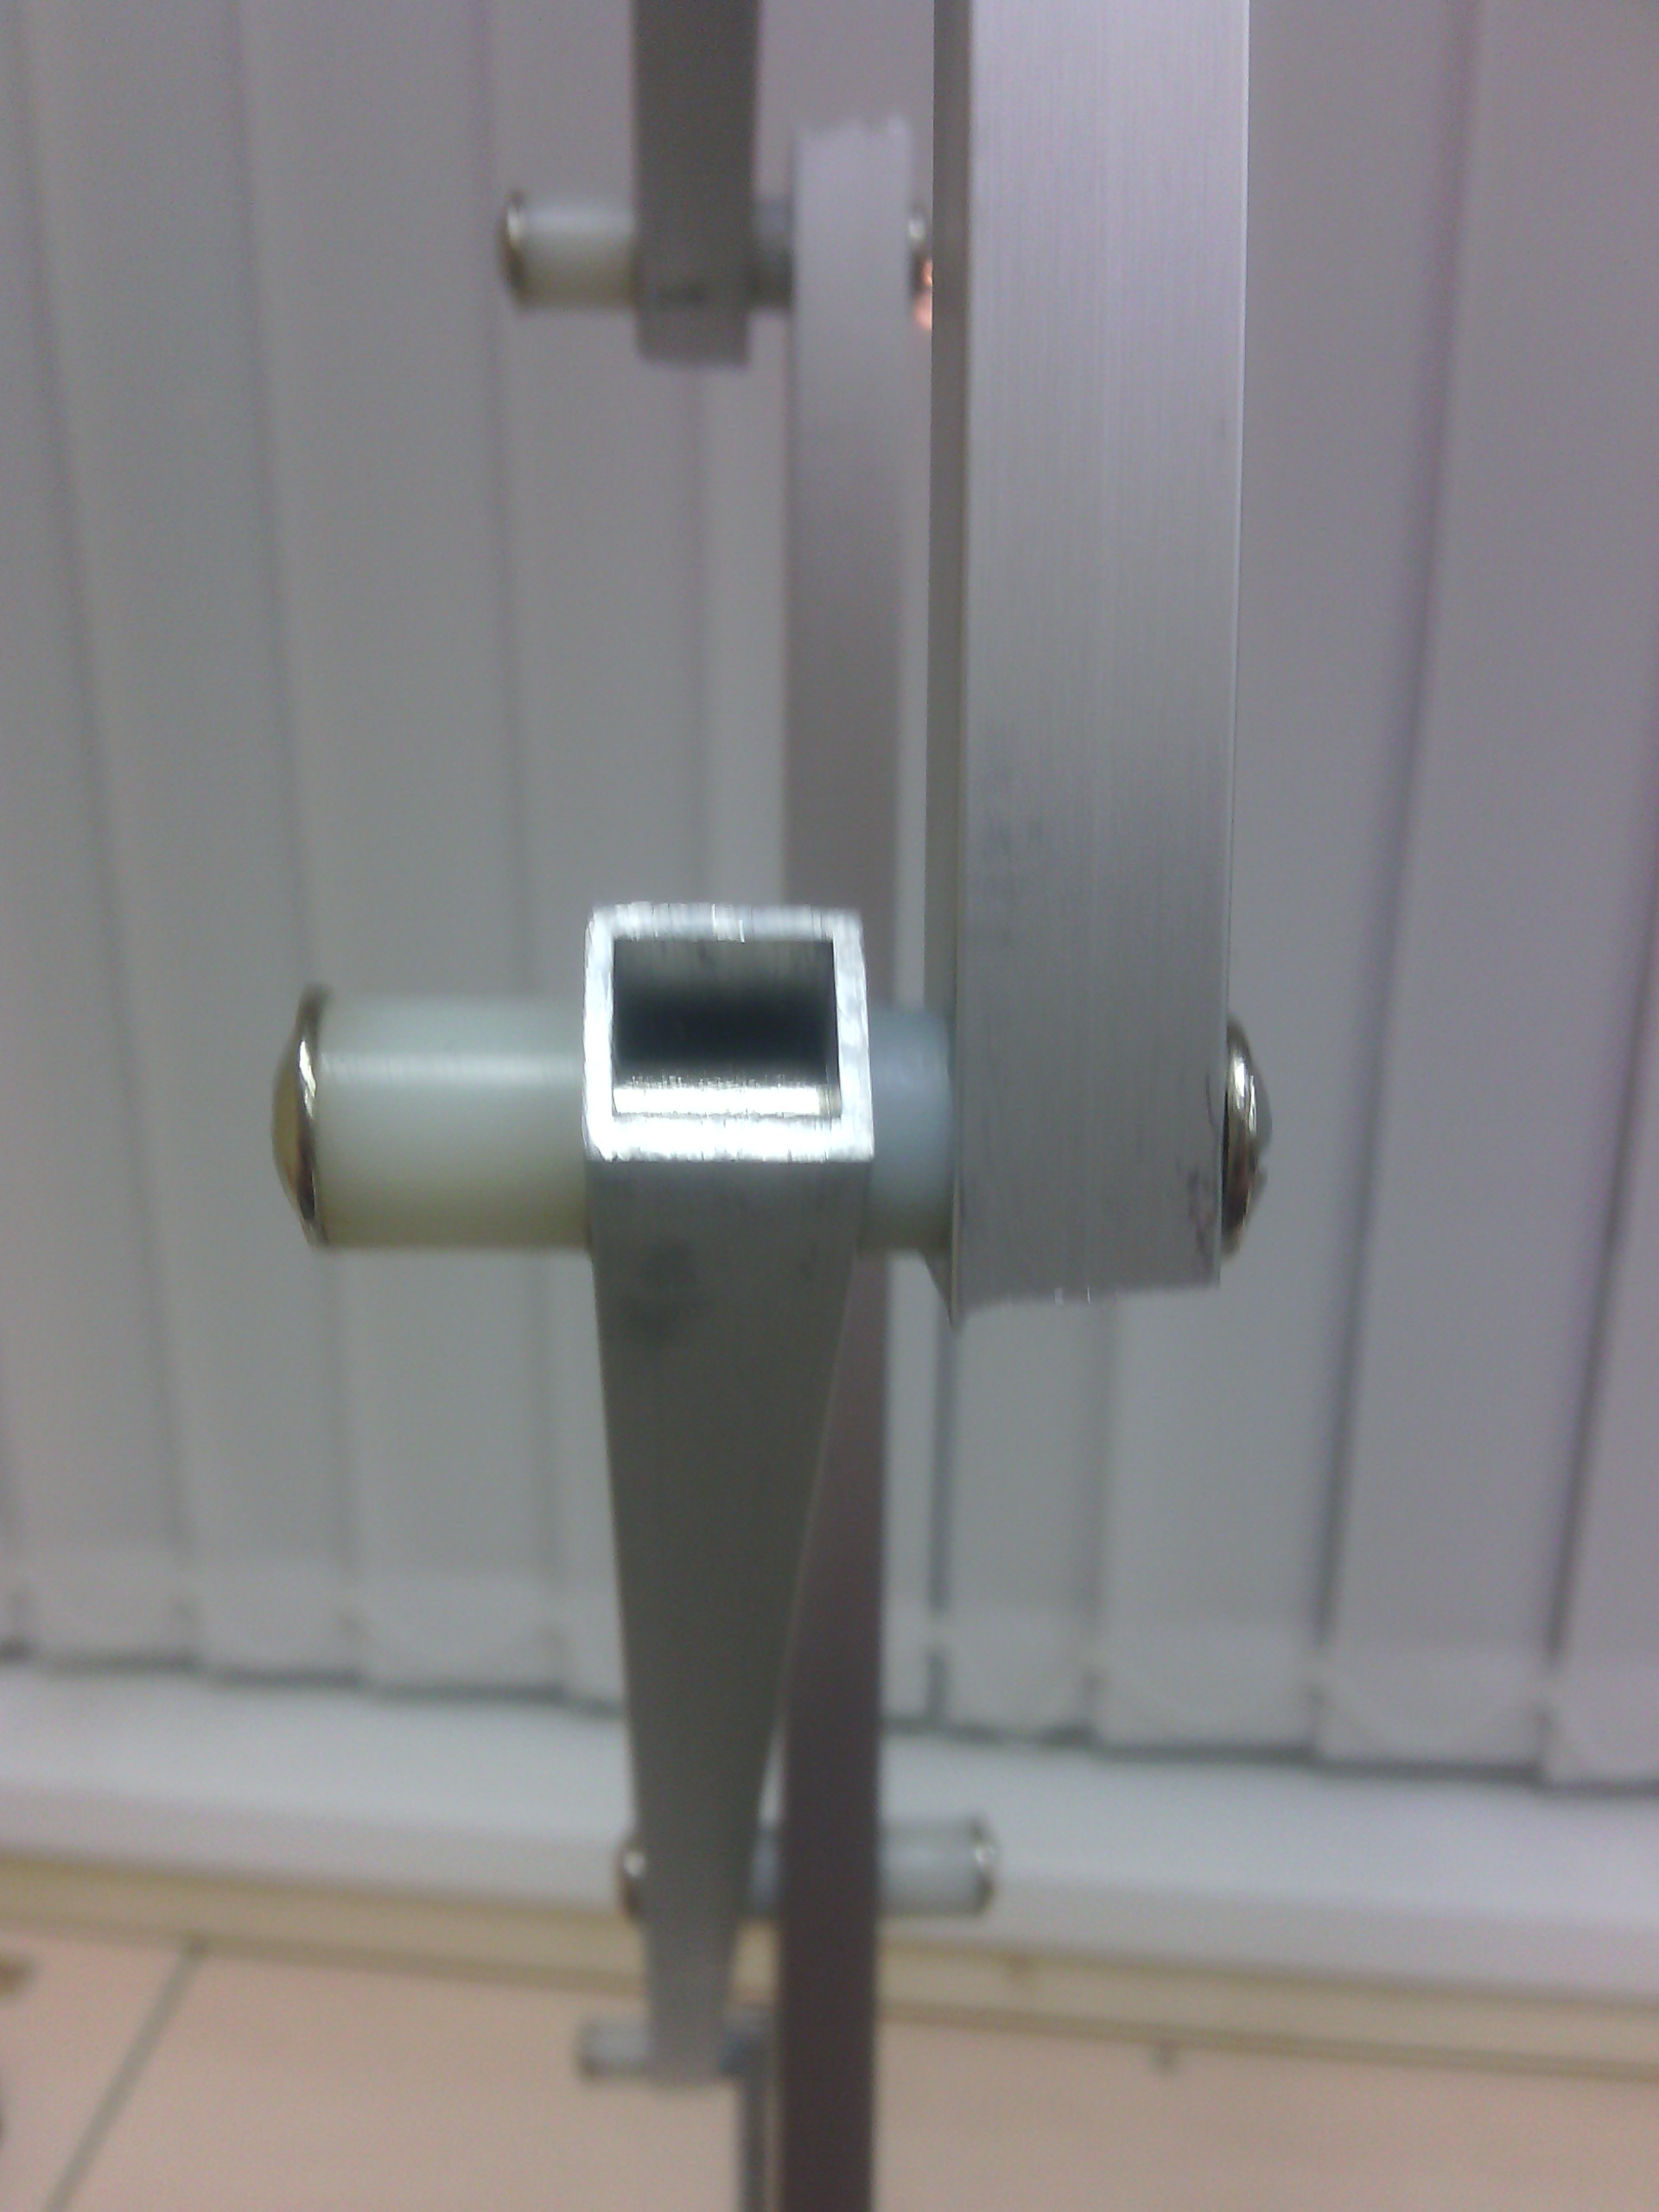
\includegraphics[width=35mm,height=35mm]{/!my_data/projects/pml30-psi_team/Days/24.10.14/10_2_robot}\\ Рисунок 12
			\end{minipage}
			\begin{minipage}{0.3\linewidth}
				\includegraphics[width=35mm,height=35mm]{/!my_data/projects/pml30-psi_team/Days/24.10.14/9_4_robot}\\ Рисунок 13
			\end{minipage}
		\end{figure}
	\end{enumerate}
\newpage